Wzorce projektowe to proste rozwiązania problemów spotykanych w programowaniu zorientowanym obiektowo\cite{wzorce}. Programowanie z użyciem wzorców wymaga większych nakładów pracy przy tworzeniu programu, jednak stworzony kod jest bardziej elastyczny na potencjalne modyfikacje.

\subsection*{Fabryka}
Ten wzorzec konstrukcyjny został użyty do budowania klas pobierających dane o odległościach z serwisów zewnętrznych. Poszczególne ich rodzaje powstały jako osobne klasy implementujące wspólny interfejs \texttt{IDistanceService}.

Wydzielenie tworzenia klas do klasy fabrycznej umożliwia łatwe dodanie kolejnych źródeł danych. Ponieważ obiekty są tworzone w jednej metodzie o nazwie \texttt{DistanceServiceFactory.Build()}, dodanie obsługi kolejnej klasy nie będzie wymagało modyfikacji każdego miejsca w kodzie korzystającego z pobierania danych.

Do klasy \texttt{DistanceServiceFactory} jest wstrzykiwany obiekt zawierający konfigurację aplikacji, na podstawie której klasa konstruuje odpowiedni typ.

\begin{figure}[htbp]
	\centering
	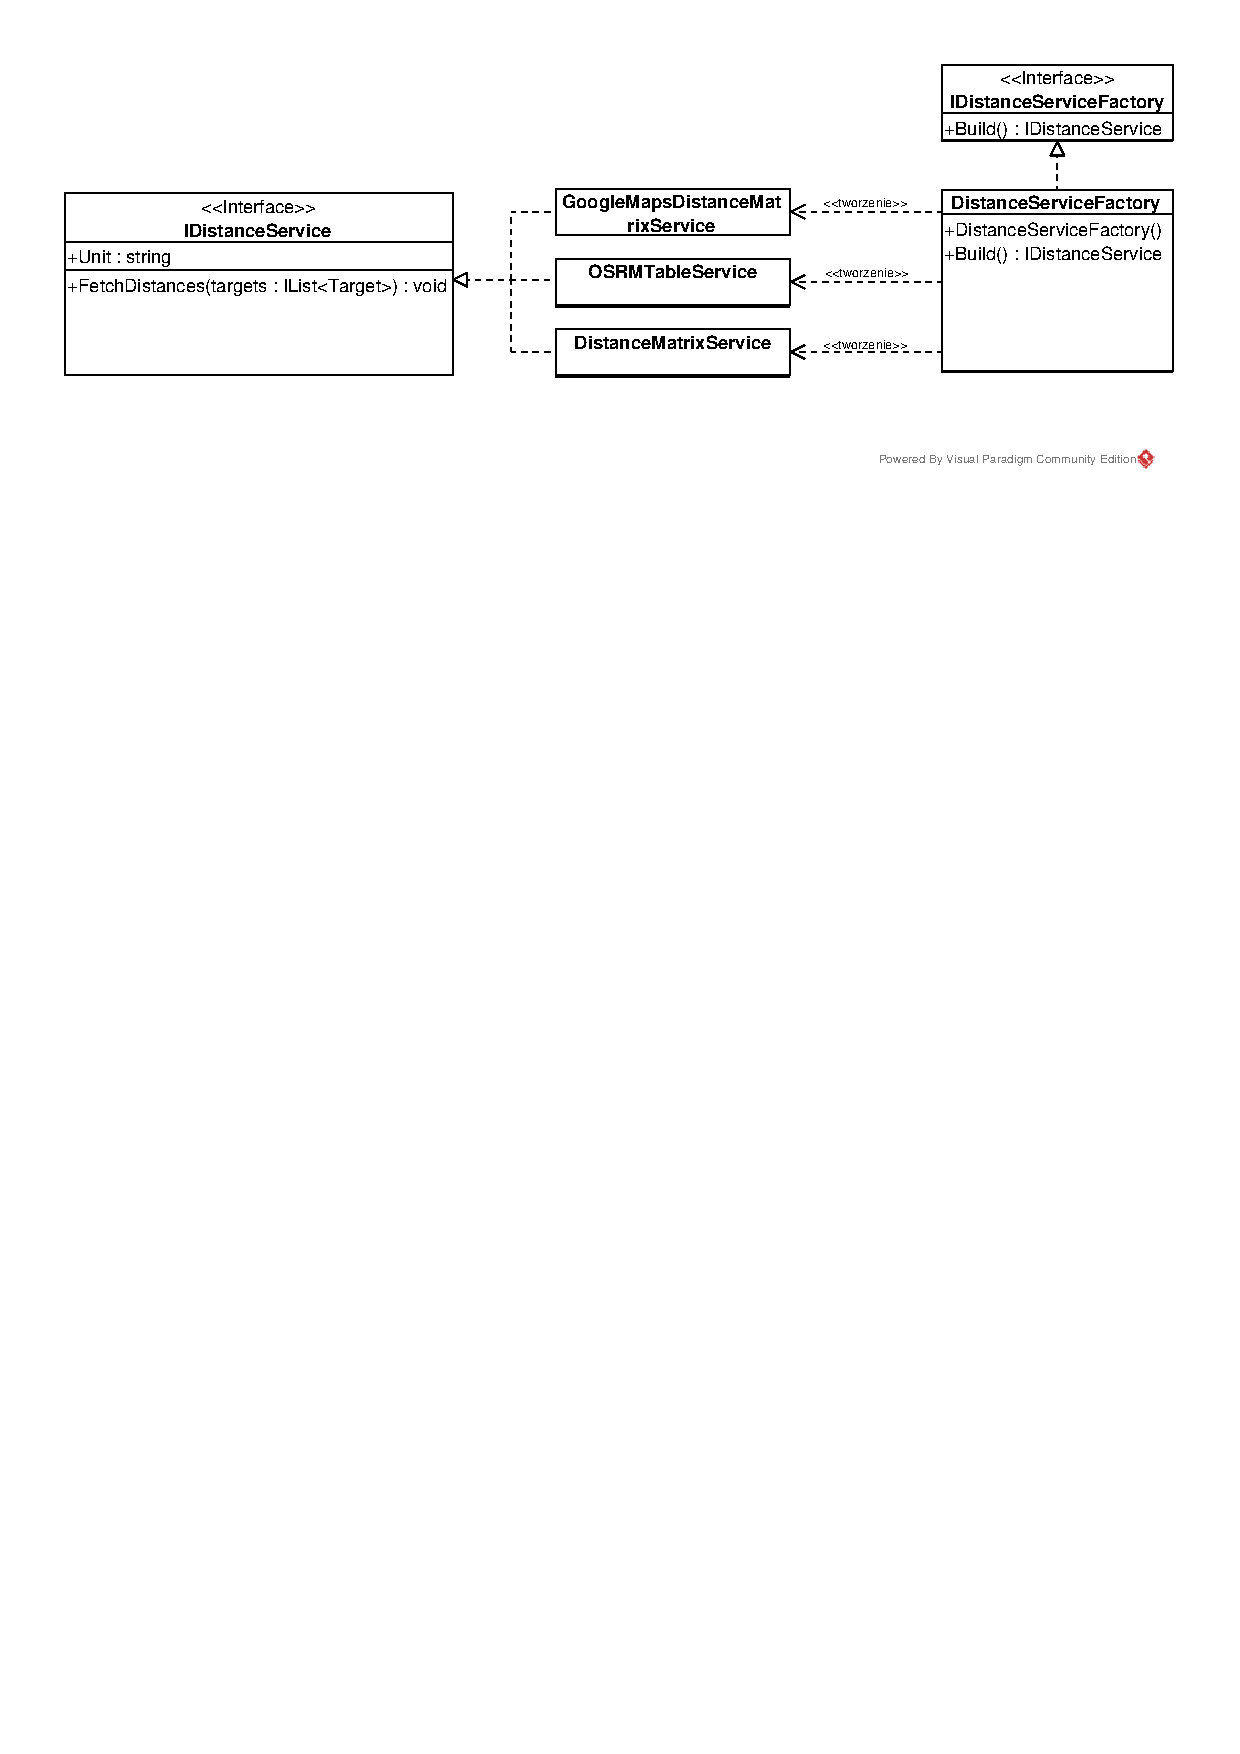
\includegraphics[clip, trim=1cm 23cm 1cm 1cm, width=1.00\textwidth]{uml/fabryka.pdf}
	\caption{Diagram klas fabryki konstruującej klasy pobierające dane zewnętrzne}
	\source{Opracowanie własne na podstawie \cite{wzorce}}
	\label{fig:fabryka}
\end{figure}

\subsection*{MVC}
Wzorzec MVC składa się z trzech typów obiektów: Modelu (\textit{Model}), Widoku (\textit{View}) i Kontrolera (\textit{Controller}). MVC pozwala na oddzielenie widoku użytkownika od warstwy przetwarzania. 

W aplikacji ten wzorzec został użyty do wyświetlenia strony głównej i~ustawień (schemat na rysunku \ref{fig:mvc}). Całym mechanizmem zarządza kontroler \texttt{HomeController}. Dziedziczy po standardowej w ASP.NET klasie abstrakcyjnej \texttt{Controller}.

\texttt{HomeController} ma dwie publiczne metody: \texttt{Index()} i \texttt{Settings()}, które służą odpowiednio do wyświetlenia strony głównej oraz podstrony zarządzania konfiguracją. Metody te wywołują konstruktory odpowiednich widoków, które zostały stworzone w HTML z pomocą składni Razor - języka służącego do tworzenia szablonów w ASP.NET.

Kontroler korzysta z modelu opisanego przez interfejs \texttt{IConfigurationService}, który zawiera dwie metody: \texttt{Get()} i \texttt{Save(Configuration config)}. Służy on do pobierania i zapisywania danych konfiguracyjnych. Interfejs ten został zaimplementowany przez klasę \texttt{TargetsFileStorage}. Klasa ta przechowuje zserializowane dane konfiguracyjne na dysku w postaci tekstowego pliku JSON. Kontroler nie tworzy obiektu tej klasy, lecz jest on wstrzykiwany jako zależność. Umożliwia to zamianę implementacji interfejsu na inny, przykładowo korzystający z bazy danych.

\begin{figure}[htbp]
	\centering
	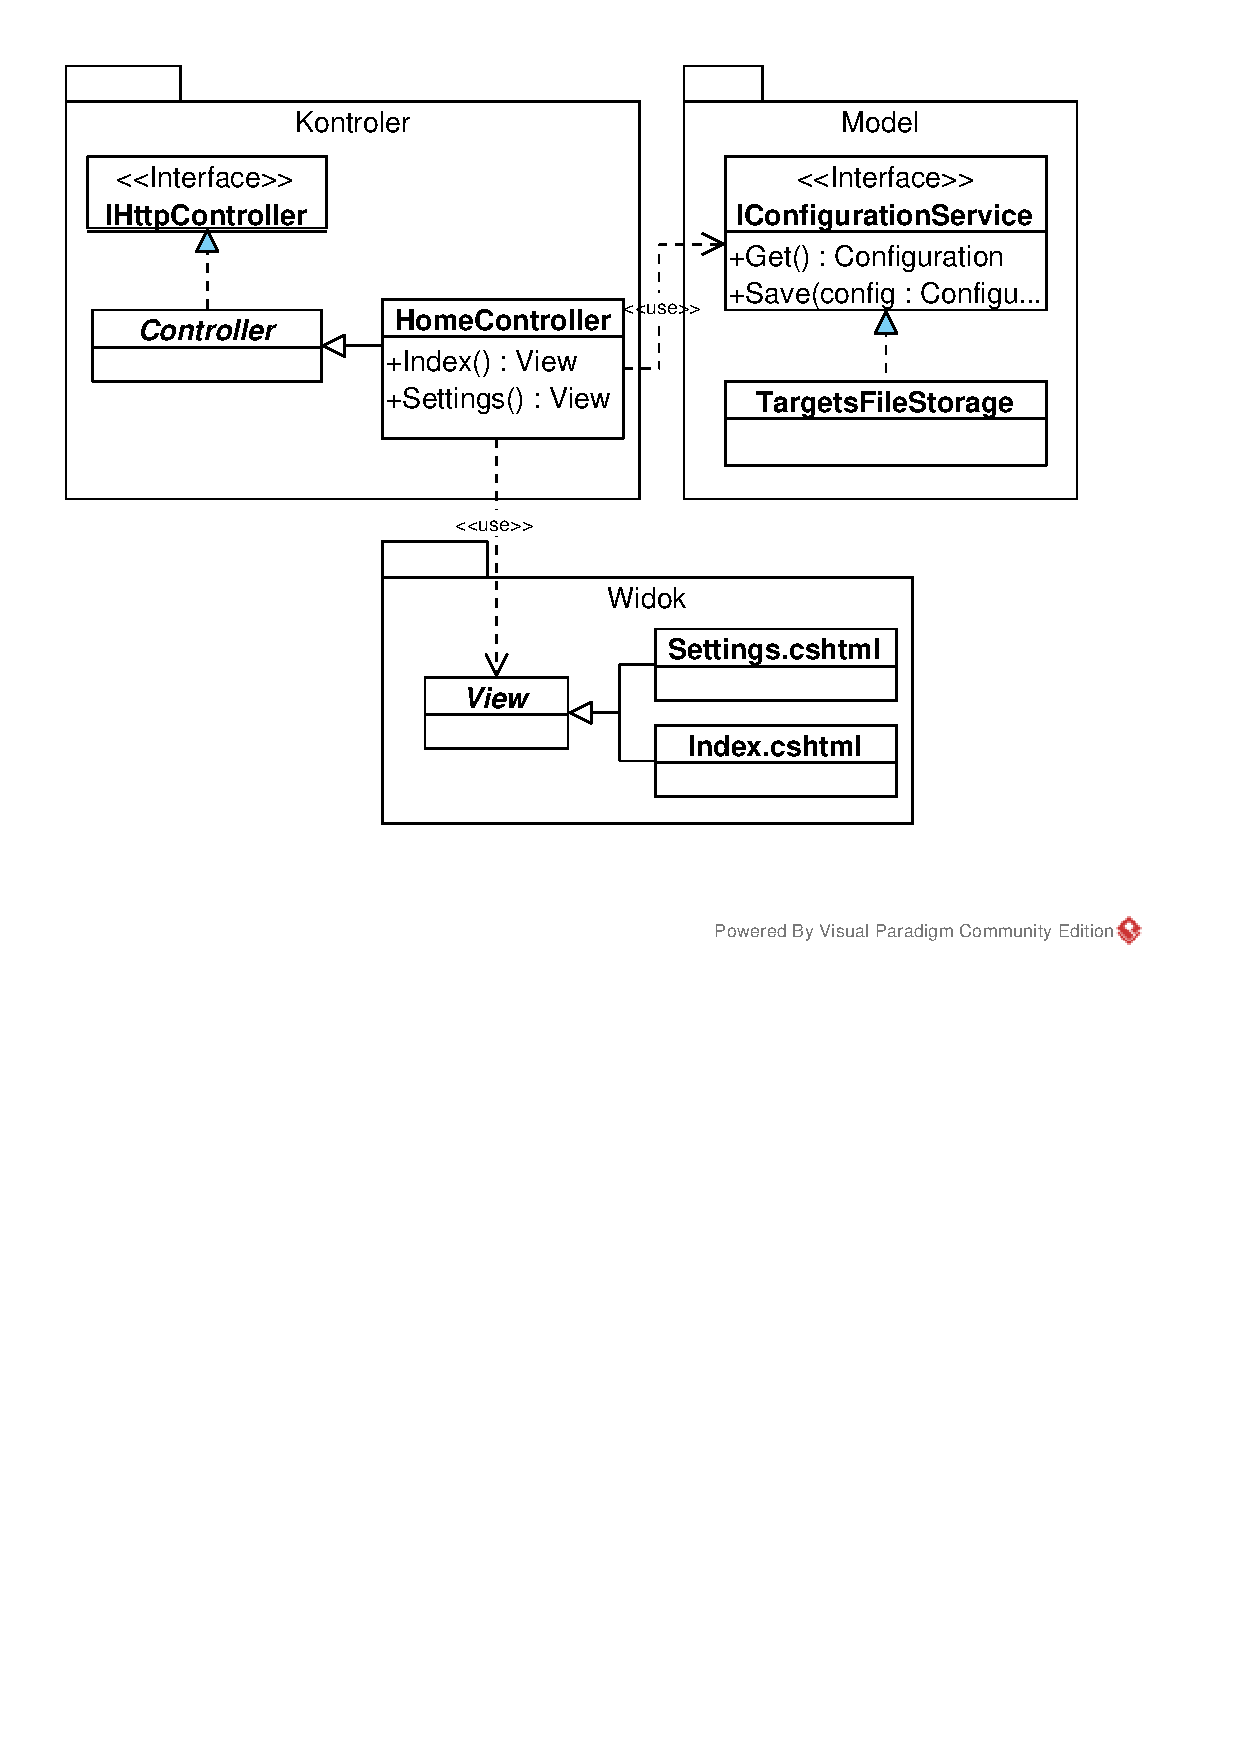
\includegraphics[clip, trim=1cm 15cm 2.5cm 1cm, width=1.00\textwidth]{uml/mvc.pdf}
	\caption{Diagram wzorca MVC w części wyświetlającej strony: główną i ustawień}
	\source{Opracowanie własne}
	\label{fig:mvc}
\end{figure}

\subsection*{Wstrzykiwanie zależności}

Wstrzykiwanie zależności (\textit{Dependency Injection}) jest wzorcem, w którym obiekty wymagane przez klasę do działania są dostarczane przez inny obiekt -- \textit{injector}. Pozwala na usunięcie bezpośredniego powiązania między klasami\cite{wstrzykiwanie}. Dzięki temu klasa korzystająca z zależności nie musi znać implementacji konkretnego obiektu, a~operować na interfejsach. Pozwala to na bezproblemową wymianę implementacji na inną.

Klasę przechowującą obiekty i przeprowadzającą wstrzykiwanie nazywa się kontenerem wstrzykiwania zależności (\textit{Dependency Injection Container}). Ponieważ kontener najczęściej zajmuje się stworzeniem obiektów, to w nim konfiguruje się czas ich życia, np. tworzenie instancji na jedno żądanie HTTP lub jedna instancja na całą aplikację (podobnie jak we wzorcu Singleton).

Mechanizm wstrzykiwania jest wspierany w ASP.NET po odpowiedniej konfiguracji. Aplikacja korzysta z gotowego kontenera o nazwie Unity. Pozwala on na wstrzykiwanie zależności do parametrów konstruktora.

Wszystkie kontrolery w opisywanej aplikacji mają zależności wstrzykiwane przez kontener.

\begin{figure}[htbp]
	\centering
	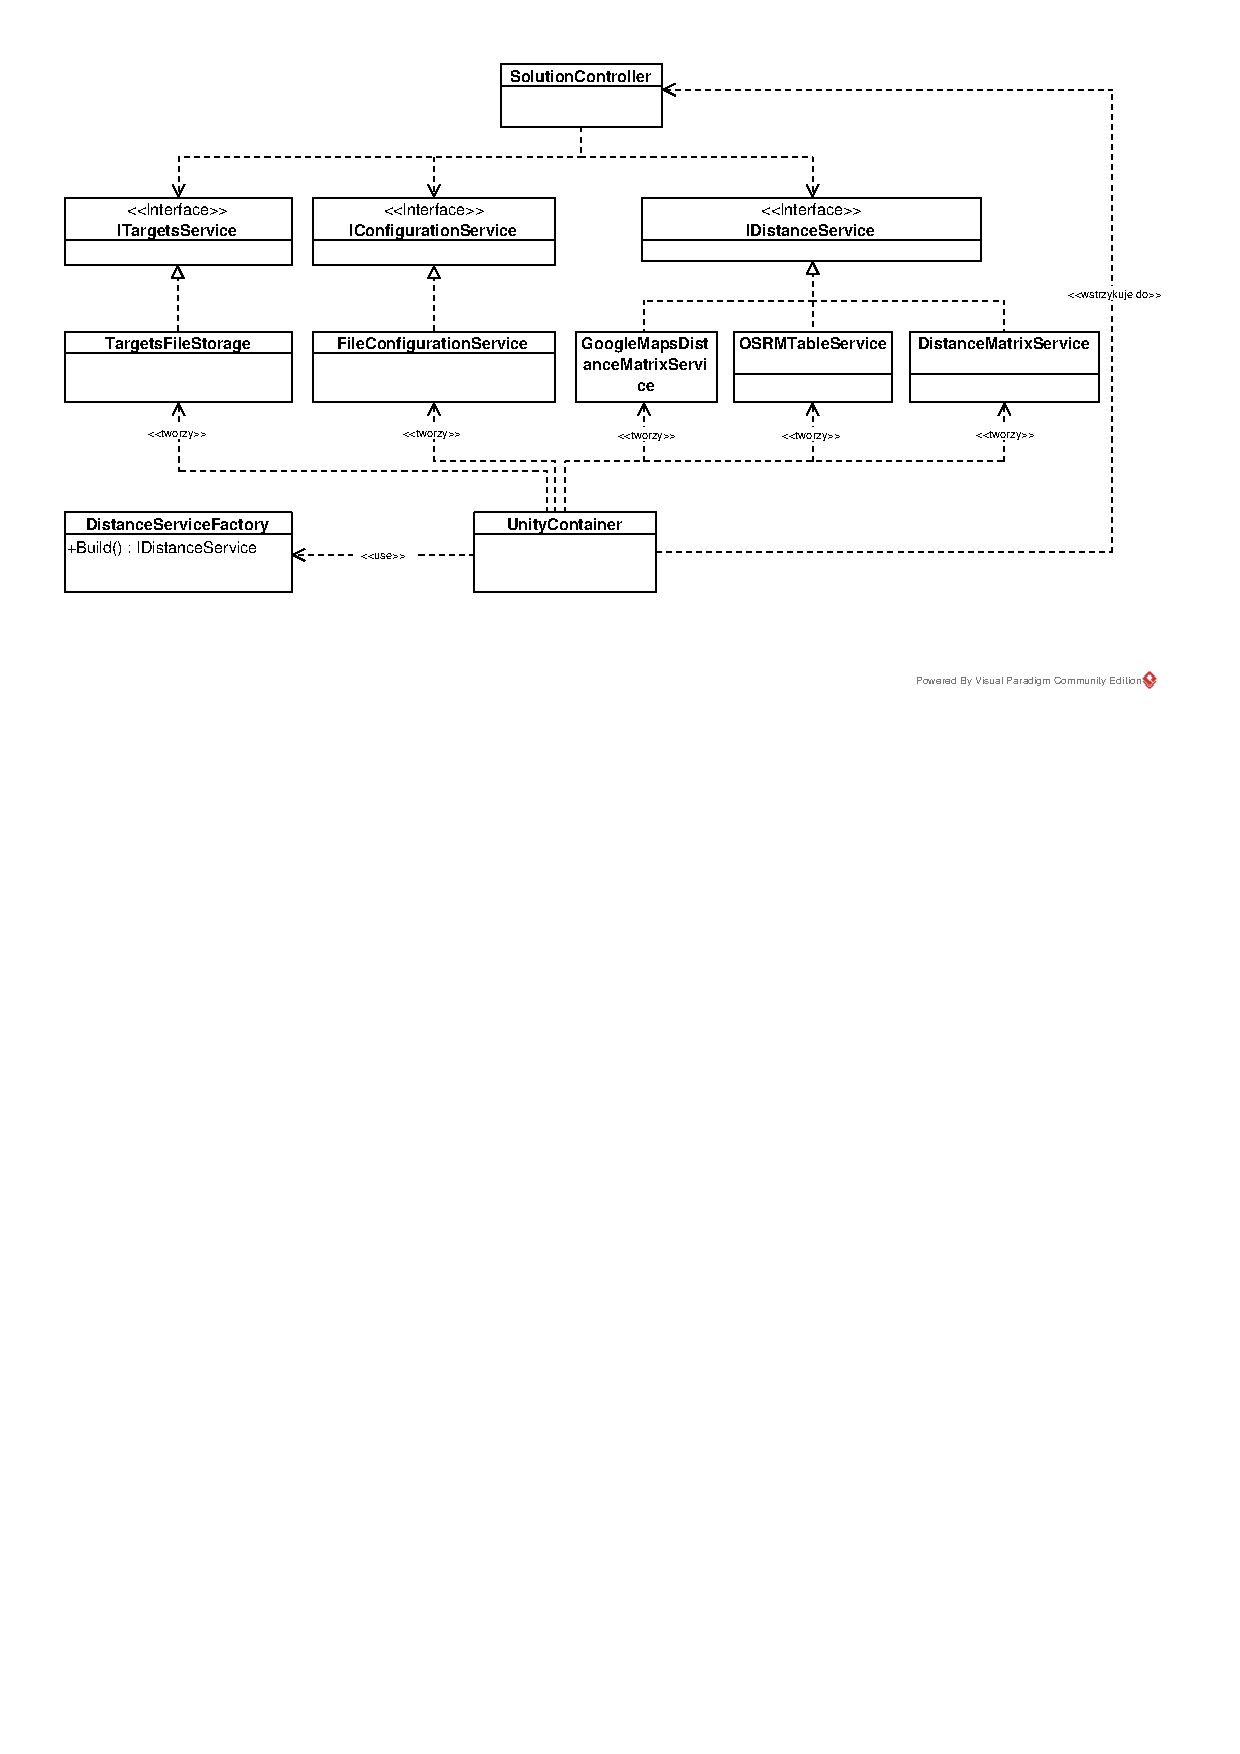
\includegraphics[clip, trim=1cm 19cm 1cm 1cm, width=1.00\textwidth]{uml/injection.pdf}
	\caption{Diagram wstrzykiwania zależności kontrolera}
	\source{Opracowanie własne na podstawie \cite{wstrzykiwanie}}
	\label{fig:di}
\end{figure}

Na rysunku \ref{fig:di} został przedstawiony schemat wstrzykiwania zależności klasy \texttt{SolutionController}. Konstruktor tego kontrolera przyjmuje trzy parametry jako interfejsy. Kontener \texttt{UnityContainer} rozwiązuje zależności wyszukując obiekt implementujący dany interfejs. Ponieważ wszystkim klasom wystarczy jedna instancja na czas działania programu, obiekty zostały uprzednio utworzone przez kontener podczas startu aplikacji.

Klasy implementujące interfejs \texttt{IDistanceService} są tworzone przez wcześniej opisaną fabrykę, natomiast pozostałe zależności są konstruowane bezpośrednio przez kontener.

\clearpage